\documentclass{article}

% packages
\usepackage{amsmath, amsthm, thmtools, amsfonts, amssymb, luacode, catchfile, tikzducks, hyperref, ifthen}
\ifcsname c@kobocompile\endcsname
	\usepackage[a5paper, total={1072pt, 1448pt}, margin=10pt, includeheadfoot]{geometry} % set page margins
\else
	\usepackage[a4paper, margin=50pt, includeheadfoot]{geometry}
\fi
\usepackage[shortlabels]{enumitem}
\usepackage[skip=3pt, indent=0pt]{parskip}

% language
\usepackage[bidi=basic, layout=tabular, provide=*]{babel}
\ifcsname c@english\endcsname
	\babelprovide[main, import]{english}
\else
	\babelprovide[main, import]{hebrew}
	\babelprovide{rl}
\fi
%\babelfont{rm}{Libertinus Serif}
\babelfont{rm}[Renderer=Harfbuzz]{Libertinus Serif}
\babelfont{sf}{Libertinus Sans}
\babelfont{tt}{Libertinus Mono}

% style
\AddToHook{cmd/section/before}{\clearpage}	% Add line break before section
\linespread{1.3}
\setcounter{secnumdepth}{0}		% Remove default number tags from sections, this won't do well with theorems
\AtBeginDocument{\setlength{\belowdisplayskip}{3pt}}
\AtBeginDocument{\setlength{\abovedisplayskip}{3pt}}
\graphicspath{ {../images/} }

% operators
\DeclareMathOperator\cis{cis}
\DeclareMathOperator\Sp{Sp}
\DeclareMathOperator\tr{tr}
\DeclareMathOperator\im{Im}
\DeclareMathOperator\re{Re}
\DeclareMathOperator\diag{diag}
\DeclareMathOperator*\lowlim{\underline{lim}}
\DeclareMathOperator*\uplim{\overline{lim}}
\DeclareMathOperator\rng{rng}
\DeclareMathOperator\Sym{Sym}
\DeclareMathOperator\Arg{Arg}
\DeclareMathOperator\Log{Log}
\DeclareMathOperator\dom{dom}
\DeclareMathOperator\supp{Supp}
\DeclareMathOperator\var{Var}
\DeclareMathOperator\cov{Cov}

% commands
%\renewcommand\qedsymbol{\textbf{מש''ל}}
%\renewcommand\qedsymbol{\fbox{\emoji{lizard}}}
\newcommand{\Aa}[0]{\mathcal{A}}
\newcommand{\Bb}[0]{\mathcal{B}}
\newcommand{\CC}[0]{\mathbb{C}}
\newcommand{\Cc}[0]{\mathcal{C}}
\newcommand{\EE}[0]{\mathbb{E}}
\newcommand{\FF}[0]{\mathbb{F}}
\newcommand{\Ff}[0]{\mathcal{F}}
\newcommand{\Ii}[0]{\mathcal{I}}
\newcommand{\Gg}[0]{\mathcal{G}}
\newcommand{\Ll}[0]{\mathcal{L}}
\newcommand{\Mm}[0]{\mathcal{M}}
\newcommand{\NN}[0]{\mathbb{N}}
\newcommand{\Nn}[0]{\mathcal{N}}
\newcommand{\PP}[0]{\mathbb{P}}
\newcommand{\Pp}[0]{\mathcal{P}}
\newcommand{\QQ}[0]{\mathbb{Q}}
\newcommand{\RR}[0]{\mathbb{R}}
\newcommand{\Rr}[0]{\mathcal{R}}
\newcommand{\Ss}[0]{\mathcal{S}}
\newcommand{\TT}[0]{\mathbb{T}}
\newcommand{\Uu}[0]{\mathcal{U}}
\newcommand{\Vv}[0]{\mathcal{V}}
\newcommand{\Ww}[0]{\mathcal{W}}
\newcommand{\ZZ}[0]{\mathbb{Z}}
\newcommand{\acts}[0]{\circlearrowright}
\newcommand{\explain}[2] {
	\begin{flalign*}
		 && \text{#2} && \text{#1}
	\end{flalign*}
}
\newcommand{\maketitleprint}[0]{ \begin{center}
	%\begin{tikzpicture}[scale=3]
	%	\duck[graduate=gray!20!black, tassel=red!70!black]
	%\end{tikzpicture}	
	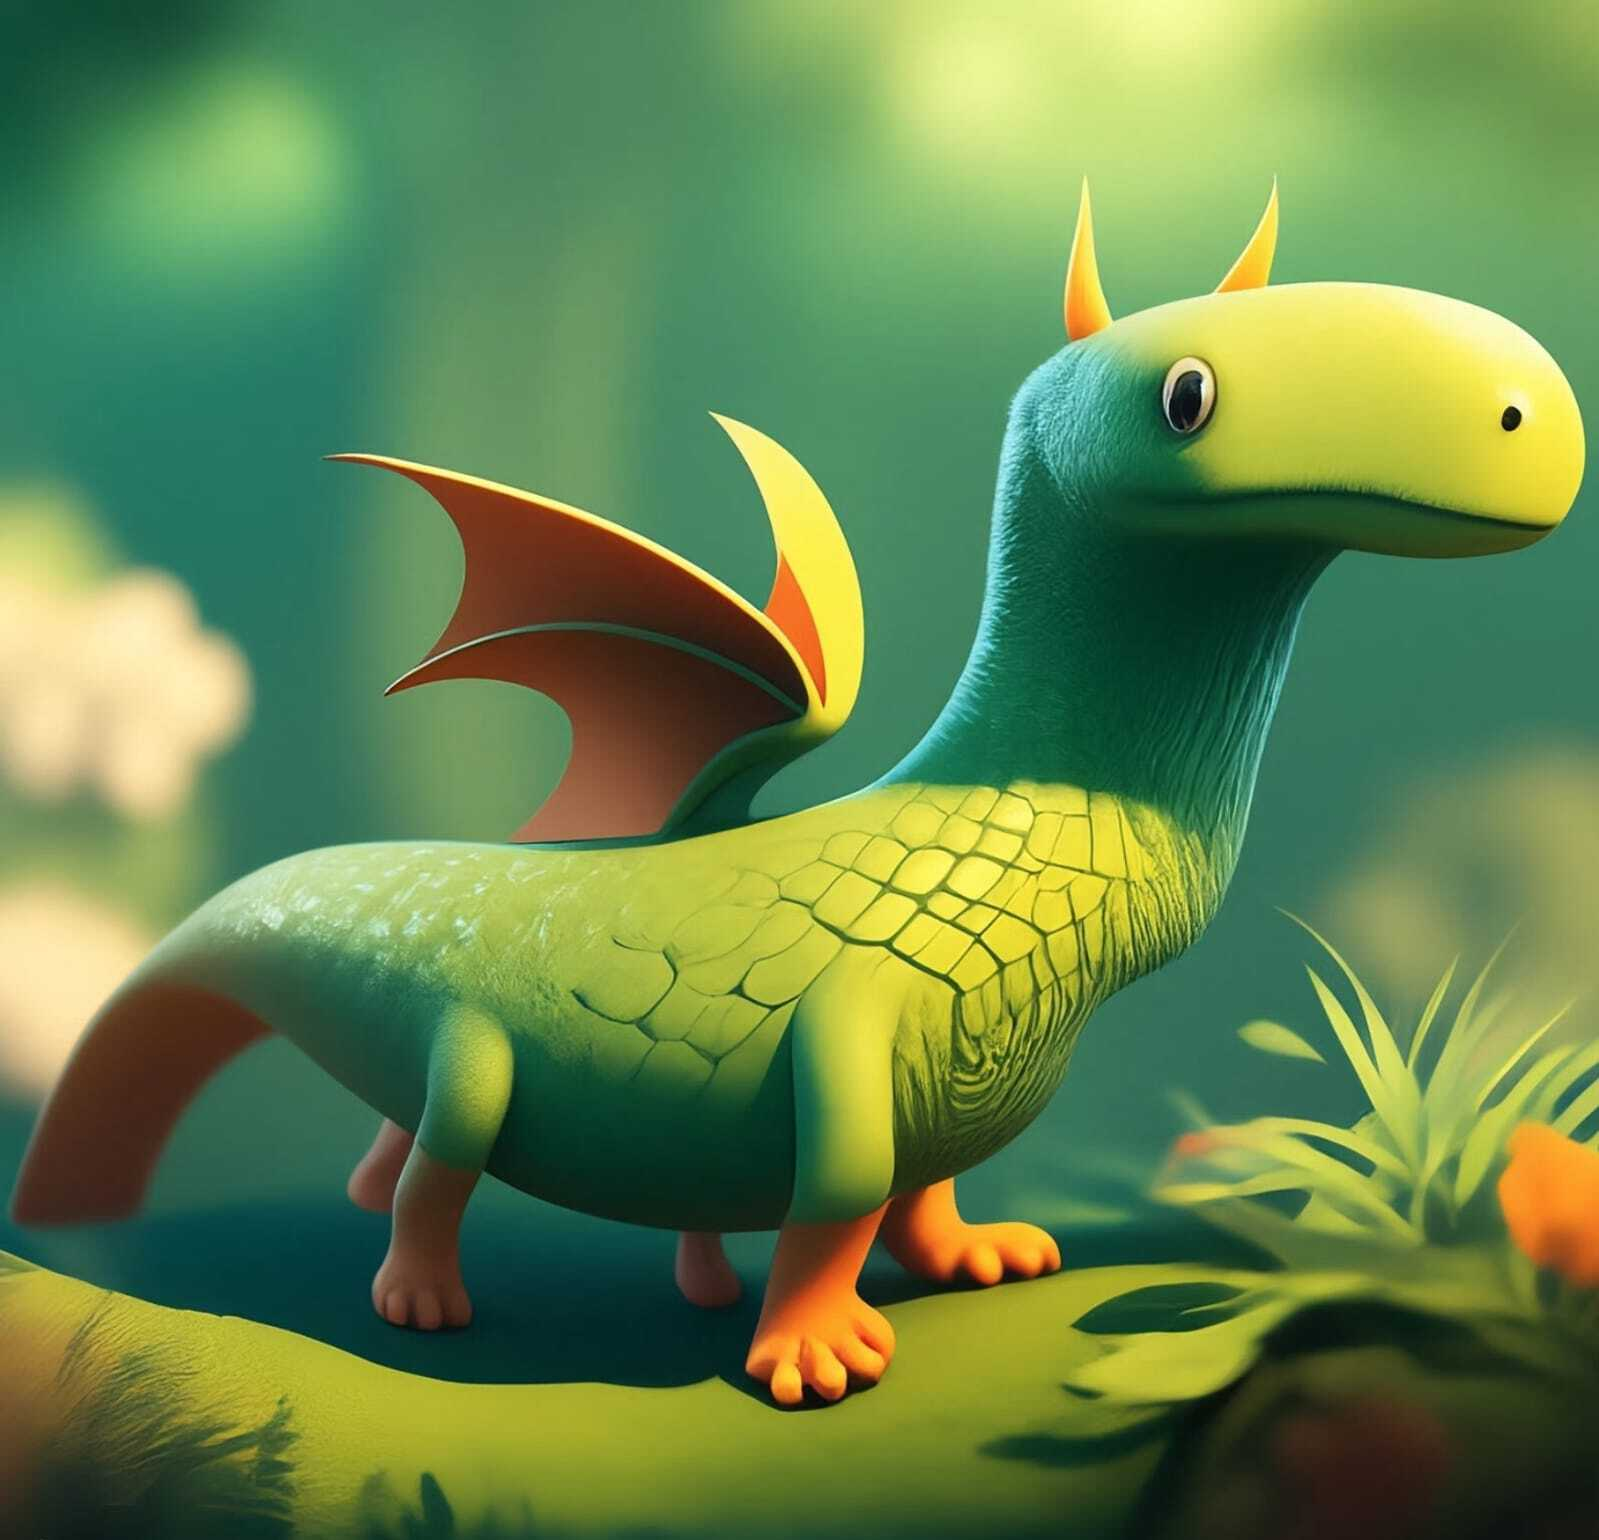
\includegraphics[width=6cm]{cover}
\end{center}
}

% theorem commands
\newtheoremstyle{c_remark}
	{}	% Space above
	{}	% Space below
	{}% Body font
	{}	% Indent amount
	{\bfseries}	% Theorem head font
	{}	% Punctuation after theorem head
	{.5em}	% Space after theorem head
	{\thmname{#1}\thmnumber{ #2}\thmnote{ \normalfont{\text{(#3)}}}}	% head content
\newtheoremstyle{c_definition}
	{3pt}	% Space above
	{3pt}	% Space below
	{}% Body font
	{}	% Indent amount
	{\bfseries}	% Theorem head font
	{}	% Punctuation after theorem head
	{.5em}	% Space after theorem head
	{\thmname{#1}\thmnumber{ #2}\thmnote{ \normalfont{\text{(#3)}}}}	% head content
\newtheoremstyle{c_plain}
	{3pt}	% Space above
	{3pt}	% Space below
	{\itshape}% Body font
	{}	% Indent amount
	{\bfseries}	% Theorem head font
	{}	% Punctuation after theorem head
	{.5em}	% Space after theorem head
	{\thmname{#1}\thmnumber{ #2}\thmnote{ \text{(#3)}}}	% head content

\ifcsname c@english\endcsname
	\theoremstyle{plain}
	\newtheorem{theorem}{Theorem}[section]
	\newtheorem{lemma}[theorem]{Lemma}
	\newtheorem{proposition}[theorem]{Proposition}
	\newtheorem*{proposition*}{Proposition}
	%\newtheorem{corollary}[theorem]{אין חלופה עברית}

	\theoremstyle{definition}
	\newtheorem{definition}[theorem]{Definition}
	\newtheorem*{definition*}{Definition}
	\newtheorem{example}{Example}[section]
	\newtheorem{exercise}{Exercise}[section]

	\theoremstyle{remark}
	\newtheorem*{remark}{Remark}
	\newtheorem*{solution}{Solution}
	\newtheorem{conclusion}[theorem]{Conclusion}
	\newtheorem{notation}[theorem]{Notation}
\else
	\theoremstyle{c_plain}
	\newtheorem{theorem}{משפט}[section]
	\newtheorem{lemma}[theorem]{למה}
	\newtheorem{proposition}[theorem]{טענה}
	\newtheorem*{proposition*}{טענה}
	%\newtheorem{corollary}[theorem]{אין חלופה עברית}

	\theoremstyle{c_definition}
	\newtheorem{definition}[theorem]{הגדרה}
	\newtheorem*{definition*}{הגדרה}
	\newtheorem{example}{דוגמה}[section]
	\newtheorem{exercise}{תרגיל}[section]

	\theoremstyle{c_remark}
	\newtheorem*{remark}{הערה}
	\newtheorem*{solution}{פתרון}
	\newtheorem{conclusion}[theorem]{מסקנה}
	\newtheorem{notation}[theorem]{סימון}
\fi

% Questions related commands
\newcounter{question}
\setcounter{question}{1}
\newcounter{sub_question}
\setcounter{sub_question}{1}

\ifcsname c@english\endcsname
	\newcommand{\question}[1][0]{
		\ifthenelse{#1 = 0}{}{\setcounter{question}{#1}}
		\section{Question \arabic{question}}
		\addtocounter{question}{1}
		\setcounter{sub_question}{1}
	}

	\newcommand{\subquestion}[1][0]{
		\ifthenelse{#1 = 0}{}{\setcounter{sub_question}{#1}}
		\subsection{Part \alph{sub_question}}
		\addtocounter{sub_question}{1}
	}
\else
	\newcommand{\question}[1][0]{
		\ifthenelse{#1 = 0}{}{\setcounter{question}{#1}}
		\section{שאלה \arabic{question}}
		\addtocounter{question}{1}
		\setcounter{sub_question}{1}
	}

	\newcommand{\subquestion}[1][0]{
		\ifthenelse{#1 = 0}{}{\setcounter{sub_question}{#1}}
		\subsection{סעיף \localecounter{letters.gershayim}{sub_question}}
		\addtocounter{sub_question}{1}
	}
\fi

% import lua and start of document
\directlua{common = require ('../common')}

\GetEnv{AUTHOR}

% headers
\author{\AUTHOR}
\date\today

\title{פתרון מטלה 01 --- תורת הקבוצות (80200)}

\begin{document}
\maketitle
\maketitleprint{}

\Question{}
\Subquestion{}
נוכיח כי אם $F$ קבוצת זוגות סדורים אז $F$ היא פונקציה אם ורק אם $\forall x, y, y': \langle x, y\rangle, \langle x, y' \rangle \in F \implies y = y'$.
\begin{proof}
	\textbf{כיוון ראשון:}
	נניח כי $F$ פונקציה. \\*
	נגדיר $F : A \to B$, לכן לכל $x \in A$ קיים זוג סדור יחיד ב־$F$ אשר רכיבו השמאלי הוא $x$. לכן נובע ישירות כי אם $\langle x, y\rangle, \langle x, y' \rangle \in F$ אז $y = y'$. \\*
	\textbf{כיוון שני:}
	נניח $\forall x, y, y': \langle x, y\rangle, \langle x, y' \rangle \in F \implies y = y'$. \\*
	נבחר $A$ קבוצת כל ה־$x$־ים המקיימים את הטענה.
	לכן $\forall x \in A \exists y : \langle x, y \rangle \in F$. \\*
	עתה נשים לב שנתון כי אם $y, y'$ מקיימים את הטענה עבור $x \in A$ כלשהו, אז $y = y'$, ולכן נובע גם
	$\forall x \in A \exists ! y : \langle x, y \rangle \in F$. \\*
	לכן $F$ היא פונקציה על־פי הגדרה.
\end{proof}

\Subquestion{}
יהיו $f, g$ פונקציות, נוכיח כי $f \cap g$ היא פונקציה.
\begin{proof}
	נגדיר $A = dom(f), B = dom(g)$. אז לכל איבר $c \in A \cap B$ מתקיים מהנתון $f(c) = g(c)$. \\*
	לכן קבוצת הזוגות הסדורים $A \cap B$ מכילה זוג סדור אחד ויחיד לכל איבר ב־$A \cap B$ ומההגדרה נקבל כי זוהי פונקציה.
\end{proof}

\Subquestion{}
נראה דוגמה לפונקציות $f, g$ כך ש־$f \cup g$ לא פונקציה: \\*
נגדיר $A = \{0, 1\}$, ואת הפונקציות $f, g : A \to A$ על־ידי
\[
	f(x) = 1, g(x) = 0
\]
ולכן נובע
\[
	f = \{(0, 1), (1, 1)\}, g = \{(0, 0), (1, 0)\}
\]
אז
\[
	f \cup g = \{(0, 1), (1, 1), (0, 0), (1, 0)\}
\]
וזוהי כמובן לא פונקציה.

\Subquestion{}
נראה דוגמה לפונקציות $f, g$ כך שמתקיים $dom(f \cap g) \ne dom(f) \cap dom(g)$. \\*
נגדיר $A$ כמו בסעיף הקודם ו־$f, g : A \to A$. נגדיר
\[
	f = \{(0, 1), (1, 0)\}, g = \{(0, 0), (1, 0)\}, f \cap g = \{(1, 0)\}
\]
לכן
\[
	dom(f \cap g) = \{1\} \ne dom(f) \cap dom(g) = \{0, 1\} \cap \{0, 1\} = \{0, 1\}
\]

\Question{}
תהי $f : A \to B$.
נוכיח כי שלושת התנאים הבאים שקולים:
\begin{enumerate}
	\item $f$ הפיכה.
	\item $f$ חד־חד ערכית ועל.
	\item קיימת פונקציה $g : B \to A$ כך ש־$f \circ g = id_B, g \circ f = id_A$.
\end{enumerate}
\begin{proof}
	\textbf{1 \leftarrow{} 2}:
	ידוע כי $f$ הפיכה ולכן $f^{-1}$ היא פונקציה. \\*
	נניח בשלילה ש־$f$ לא חד־חד ערכית ולכן קיימים $a, b \in A$ כך ש־$a \ne b, f(a) = f(b) = y$.
	לכן על־פי הגדרה נובע כי $\langle y, a \rangle, \langle y, b \rangle \in f^{-1}$.
	אבל ידוע כי $f^{-1}$ פונקציה והגענו לסתירה, לכן $f$ חד־חד ערכית. \\*
	נניח בשלילה ש־$f$ לא על, לכן קיים $y \in B$ כך ש־$\forall a \in A, \langle a, y \rangle \not\in f$. אבל ידוע ש־$f^{-1}$ פונקציה ולכן $\langle y, x \rangle \in f^{-1}$ עבור $x \in A$ כלשהו.
	זוהי סתירה ולכן $f$ חד־חד ערכית ועל. \\*
	\textbf{2 \leftarrow{} 3}:
	נניח כי $f$ חד־חד ערכית ועל, ונגדיר $g = \{ \langle y, x \rangle \mid \langle x, y \rangle \in f \}$.
	ידוע כי $f$ חד־חד ערכית, ולכן כל איבר באגף ימני של $f$ לא חוזר על עצמו ובהתאם אין חזרה באגף ימני של $g$, והיא עומדת בהגדרת פונקציה.
	נניח שקיים $b \in B$ כך ש־$g(b)$ לא מוגדר, לכן אין $a \in A$ כך ש־$f(a) = b$, אך זו סתירה להיותה של $g$ על, ולכן לא קיים $b$ כזה.
	במילים אחרות, לכל $b \in B$ מתקיים $g(b) = a$ עבור $a$ כלשהו.
	עתה נראה כי $\forall a \in A, g(f(a)) = g(b) = a$ שכן אם $\langle a, b \rangle \in f$ אז $\langle b, a \rangle \in g$.
	באופן דומה נראה כי $\forall b \in B, f(g(b)) = f(a) = b$ ולכן מתקיים $f \circ g = id_B, g \circ f = id_A$. \\*
	\textbf{3 \leftarrow{} 1}:
	נניח כי קיימת פונקציה $g : B \to A$ כך ש־$f \circ g = id_B, g \circ f = id_A$. \\*
	מהנתון נובע כי אם $\langle a, b \rangle \in f$ אז $\langle b, a\rangle \in g$, ונתון כי היא פונקציה.
	לכן גם $f^{-1} = g$.
\end{proof}

\Question{}
תהינה $f : A \to B, g : B \to C$.

\Subquestion{}
נוכיח כי אם $g, f$ הן על, אז גם $g \circ f$ היא על.
\begin{proof}
	יהי $c \in C$, $g$ היא על ולכן קיים $b \in B$ כך ש־$g(b) = c$. \\*
	ידוע כי $f$ היא על ולכן קיים $a \in A$ כך ש־$f(a) = b$, ולכן $g(f(a)) = c$ ומצאנו כי $g \circ f$ היא על.
\end{proof}

\Subquestion{}
נפריך את הטענה כי אם $g$ על אז גם $g \circ f$ על על־ידי דוגמה נגדית: \\*
נגדיר $A = B = C = \{0, 1\}$, ונגדיר $g = id_A$ ולכן על. עוד נגדיר $f(x) = 1$. \\*
נראה כי $g(f(x)) = 1$ לכל $x$ ולכן לא קיים $x$ כך ש־$g(f(x)) = 0$ ובהתאם היא לא על.

\Subquestion{}
נסתור את הטענה כי אם $g$ היא חד־חד ערכית אם $g \circ f$ היא חד־חד ערכית על־ידי דוגמה נגדית: \\*
נגדיר $A = \{0\}, B = C = \{0, 1\}$ וגם $f(0) = 0$ ו־$g(x) = 0$. \\*
ניתן להבחין כי $f$ חד־חד ערכית, וגם כי $g \circ f$ היא חד־חד ערכית, אבל $g(0) = g(1)$.

\Question{}
תהינה קבוצות $A, B, C, D$ כך שמתקיים $|A| = |C|, |B| = |D|$.

\Subquestion{}
נוכיח כי $|A \times B| = |C \times D|$.
\begin{proof}
	משוויון העוצמות נניח שיש שתי פונקציות הפיכות $f : A \to C$ ו־$g : B \to D$. \\*
	נגדיר פונקציה חדשה $h : A \times B \to B \times D$ על־ידי $h(a, b) = \langle f(a), g(b) \rangle$. \\*
	זוהי כמובן פונקציה הפיכה שכן $f, g$ הפיכות, ולכן מתקיים שוויון העוצמות $|A \times B| = |C \times D|$.
\end{proof}

\Subquestion{}
נפריך את הטענה כי $|A \cup B| = |C \cup D|$ על־ידי דוגמה נגדית: \\*
נגדיר $A = \{0, 1\}, B = \{1, 2\}, C = D = \{0, 1\}$. \\*
ברור כי כלל הקבוצות בעלות עוצמה זהה, ובפרט $|A| = |C|, |B| = |D|$, אבל $A \cup B = \{0, 1, 2\}$ ואילו $C \cup D = \{0, 1\}$ ועוצמותיהן לא שוות.

\Question{}
נוכיח כי אם $A, B$, סופיות, ו־$|A| = n, |B| = m$, אז $|A \times B| = n \cdot m$.
\begin{proof}
	נגדיר $A = [n], B = [m]$, שאם לא כן נוכל להגדיר פונקציה הפיכה בין הקבוצות ועוצמותיהן שוות, לכן לא פגענו בכלליות ההוכחה. \\*
	נשים לב כי $A \times B = \{ \langle a, b \rangle \mid 0 \le a < n, 0 \le b < m \}$ \\*
	נגדיר $C = \{ 2^a \cdot 3^b \mid 0 \le a < n, 0 \le b < m \}$, בקבוצה זו יש בדיוק $nm$ איברים. \\*
	נראה כי הפונקציה $f : A \times B \to C$ המוגדרת על־ידי $f(a, b) = 2^a 3^b$ היא חד־חד ערכית ועל ולכן נקבל כי $|A \times B| = nm$.
\end{proof}

\Question{}
\Subquestion{}
נוכיח באינדוקציה על $n \in \NN$ שאין פונקציה חד־חד ערכית מ־$[n + 1]$ ל־$[n]$.
\begin{proof}
	נבחין כי עבור $n = 1$ הפונקציה היחידה האפשרית היא $f(0) = f(1) = 0$ וזו כמובן לא חד־חד ערכית וזהו בסיס האינדוקציה. \\*
	נניח כי טענת האינדוקציה נכונה עבור $n - 1$, דהינו אין פונקצה חד־חד ערכית מ־$[n]$ ל־$[n - 1]$. \\*
	תהי פונקציה שאיננה חד־חד ערכית מ־$[n]$ ל־$[n - 1]$, ונבחן את כל הפונקציות המתקבלות ממנה על־ידי הוספת איבר לתחום ולטווח. \\*
	נבחר לייצג את הפונקציה כרשימה בתצורה $( f(0), f(1), \hdots, f(n - 1))$ ונראה כי אנו יכולים להוסיף את האיבר $n + 1$ בין כל אחד מהאיברים, והפונקציה תוגדר כ־$[n + 1] \to [n]$ ותישאר לא חד־חד ערכית. \\*
	אילו ננסה לשנות ערך קיים ברשימת הערכים להיות $n + 1$ כך שלא תהיה חד־חד ערכית, ניאלץ להוסיף מספר קיים בהוספת האיבר החדש, ונקבל שוב פונקציה לא חד־חד ערכית. \\*
	קיבלנו כי הפונקציה מ־$[n + 1]$ ל־$[n]$ היא לא חד־חד ערכית והשלמנו את מהלך האינדוקציה.
\end{proof}

\Subquestion{}
נראה כי אם $B$ סופית, $A \subseteq B$ ו־$A \ne B$ אז $A$ ו־$B$ אינן שוות עוצמה. \\*
ידוע כי $A \subseteq B$ ולכן נוכל לבנות פונקציה חד־חד ערכית מ־$A$ ל־$B$ ונקבל כי $|A| \le |B|$. \\*
ידוע כי $A \ne B$ ולכן קיים איבר אחד לפחות ב־$B$ שלא נמצא ב־$A$, וידוע כי שתי הקבוצות סופיות, נוכל להשתמש בסעיף הקודם להראות שאין פונקציה חד־חד ערכית מ־$B$ ל־$A$ ולא מתקיים $|B| \le |A|$,
לכן $|A| < |B|$ בהכרח.

\Question{}
\Subquestion{}
נוכיח את השוויון הבא:
\[
	|\{n \in \NN \mid n \equiv 0 \mod 3\}| = |\{n \in \NN \mid n \equiv 0 \mod 4\} |
\]
\begin{proof}
	נגדיר פונקציה $f$ בין הקבוצות על־ידי
	\[
		f(x) = 4x / 3, f^{-1}(x) = 3x / 4
	\]
	נבחין כי הפונקציה והפונקציה ההופכית אכן מקיימות $f \circ g = id, g \circ f = id$ ולכן הפונקציה אכן חד־חד ערכית ועל, ולכן העוצמות אכן שוות.
\end{proof}

\Subquestion{}
נוכיח את השוויון
\[
	\left\lvert \left\{ \frac{1}{1}, \frac{1}{2}, \hdots, \frac{1}{n}, \hdots \right\}\right\rvert
	= \left\lvert \left\{ \frac{1}{2}, \frac{1}{3}, \hdots, \frac{1}{n}, \hdots \right\}\right\rvert
\]
\begin{proof}
	נגדיר את הפונקציה הבאה בין הקבוצות:
	\[
		f(x) = \frac{x}{x + 1}
	\]
	כך שלכל $\frac{1}{n}$ נקבל מ־$f$ את $\frac{1}{n + 1}$. \\*
	זוהי פונקציה חד־חד ערכית ישירות מהגדרתה, ועל שכן על־פי הגדרת קבוצת הטווח אנו יכולים להגיע לכל איבר החל מהראשון (ניתן להוכיח אינדוקטיבית). \\*
	מסיבה זו עוצמת הקבוצות זהה.
\end{proof}

\Subquestion{}
נוכיח את שוויון העוצמות
\[
	|[0, 1]| = |[0, 1)| % chktex 9
\]
\begin{proof}
	נגדיר פונקציה דומה לפונקציה בסעיף הקודם, לכל $n \in \NN, n > 0$ נגדיר $f(\frac{1}{n}) = \frac{1}{n + 1}$ כל מספר ממשי אחר $f(x) = x$. \\*
	ראינו למה ההגדרה הראשונה היא חד־חד ערכית ועל לקבוצה $\{ \frac{1}{2}, \frac{1}{3}, \hdots \}$ ופונקציית הזהות היא כמובן חד־חד ערכית ועל לקבוצת הממשיים בקבוצה שאינם מהתצורה $\frac{1}{n}$ ולכן גם בכולל הקבוצה חד־חד ערכית ועל. \\*
	לכן העוצמות אכן שוות.
\end{proof}

\end{document} % chktex 17
